%\documentclass[main]{subfiles}
%\begin{document}

\chapter{Aplicación con cámara}
\label{chap:camara}

La idea principal de la aplicación consiste en implementar un método para determinar la posición del cuadricóptero utilizando una cámara filmadora. Surge como una solución a la necesidad de obtener una realimentación de posición estando a puertas cerradas, donde la señal del GPS es muy débil o directamente nula. A su vez es posible obtener una medida de los ángulos pitch, roll y yaw.\\

\begin{wrapfigure}{l}{0.55\textwidth}
	\begin{center}
		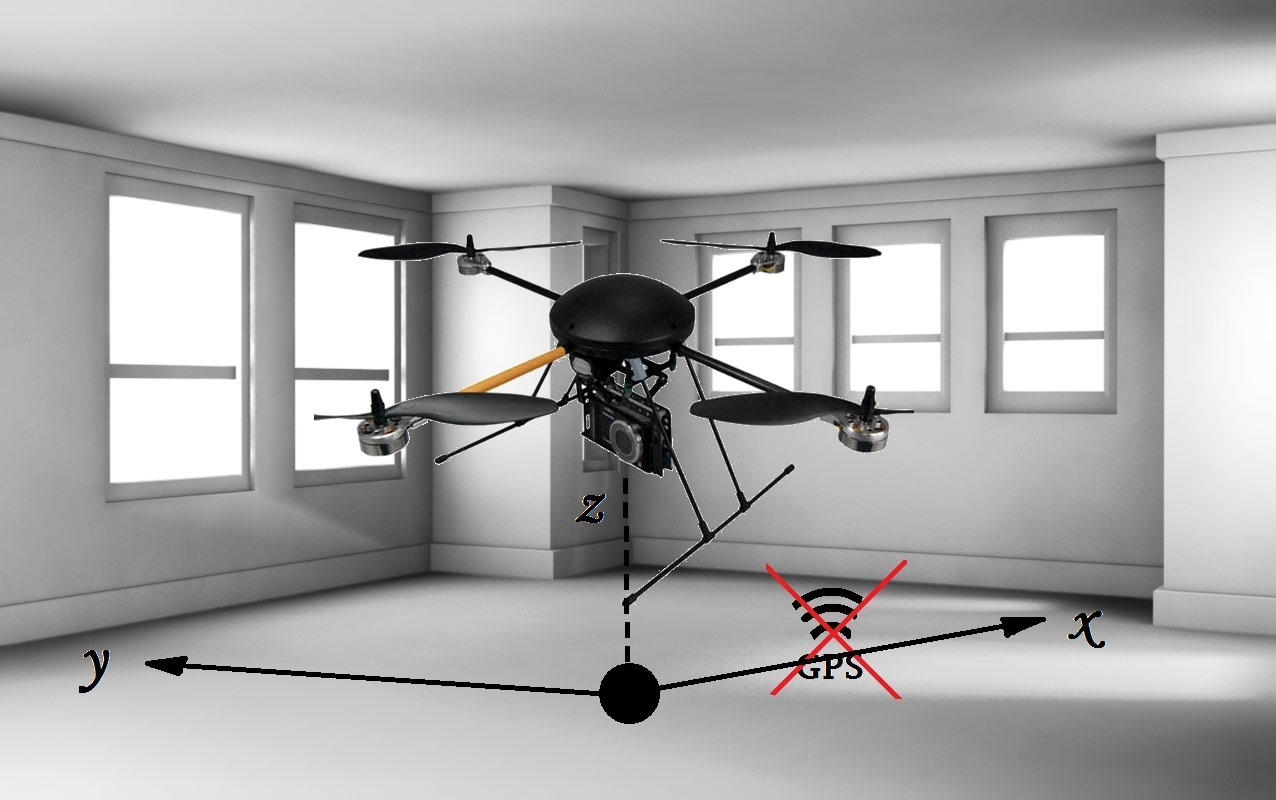
\includegraphics[width=0.5\textwidth]{./pics_camara/presentacion.jpg}
	\end{center}
	\caption{Presentación de la aplicación}
	\label{fig:presentacion}
\end{wrapfigure}

En la figura \ref{fig:presentacion} se observa un diagrama que representa al problema a solucionar. Se desean hallar los parámetros de posición ``$x$'', ``$y$'' y ``$z$'' y los parámetros de orientación: $roll$, $pitch$ y $yaw$, mediante la identificación de algunos marcadores cuya posición y orientación es conocida.\\

Se consideran distintos patrones (marcadores) para identificar las distintas paredes de una habitación. Los patrones son reconocidos e identificados para luego, conociendo los parámetros intrínsecos de la cámara, obtener la posición espacial de la cámara respecto a cada patrón. La ubicación de los patrones respecto a la habitación es conocida, deduciendo así la posición del UAV en la habitación. Una vez detectados e identificados los marcadores, se halla la transformación que lleva el sistema de coordenadas referenciado en el marcador al sistema de coordenadas referenciado en la cámara, obteniéndose una matriz de rotación \textbf{R} y un vector de traslación \textbf{T}, los cuales describen completamente la posición relativa entre la cámara y el marcador.\\

Para poder determinar los 6 grados de libertad que tiene el problema son necesarios al menos 3 puntos de correspondencia entre las coordenadas del mundo (3D) y las de la foto (2D), aunque cuantos más puntos se tengan, mejores serán los resultados obtenidos.\\

Es importante destacar que el algoritmo debe ser lo suficientemente rápido como para procesar las imágenes en tiempo real. El cuadricóptero equipado con la cámara estará filmando en todo momento y es necesario obtener la posición en todo momento sin un retardo demasiado grande. Es evidente que puede ocurrir que durante varios frames no se tenga ningún marcador a la vista, situación en la que se confiará plenamente en la estimación del estado obtenida del filtro de Kalman. Para la estimación de los ángulos esta situación no es tan grave, ya que se puede obtener realimentación mediante el acelerómetro y el giróscopo, pero para la estimación de la posición se deberá confiar únicamente en la predicción realizada por el filtro, sin realimentación alguna.

\section{Sistemas de coordenadas}

Es importante definir algunas convenciones que se utilizarán más adelante para poder entender la aplicación. Por ello se aclaran los sistemas de coordenadas utilizados.\\

Por un lado se tienen las coordenadas del ``mundo'', representadas en la figura \ref{fig:coordenadas} como ``$i$'', ``$j$'' y ``$k$'', que son coordenadas espaciales (3D). Por otro lado, también representadas en la figura, están las coordenadas de la cámara que también son espaciales y se representan mediante ``$ic$'', ``$jc$'' y ``$kc$''.

\begin{wrapfigure}{l}{0.55\textwidth}
	\begin{center}
		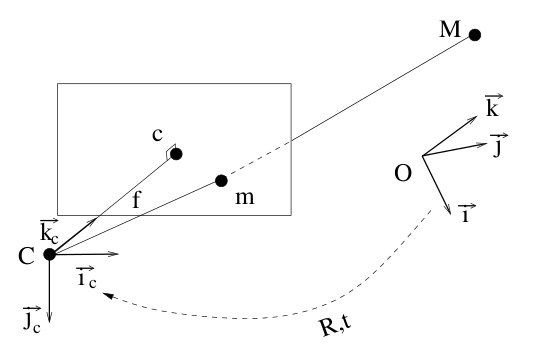
\includegraphics[width=0.5\textwidth]{./pics_camara/coordenadas.jpg}
	\end{center}
	\caption{Sistemas de coordenadas}
	\label{fig:coordenadas}
\end{wrapfigure}

Además, y no menos importantes están las coordenadas de la foto. Son coordenadas en el plano y por lo tanto en 2 dimensiones. ``$M$'' representa un punto en el espacio con coordenadas ``en el mundo'' según $(i,j,k)$. A su vez es posible expresar las coordenadas de ``$M$'' en el marco de referencia de la cámara según los versores $(ic,jc,kc)$.\\

El pasaje entre las coordenadas "del mundo" y las coordenadas "de la cámara" se realiza mediante la rotación R y la translación T.
Siendo ``$X$'' las coordenadas del mundo de ``$M$'' y ``$X_c$'' las coordenadas de ``$M$'' referenciadas a la cámara. Entonces se puede afirmar:
$$X_c = R X + T$$

``$m$'' es la proyección de ``$M$'' en el plano de la imagen, llevando coordenadas en el plano (2D). ``$c$'' es el punto principal y ``$f$'' la distancia focal.

\section{Marcadores}

El marcador consta básicamente de 3 bloques de cuadrados concéntricos. $El 4^o$ lugar será ocupado por algún identificador para diferenciar distintos marcadores. El hecho de que tenga 3 bloques en 3 esquinas distintas permite conocer con facilidad la orientación del mismo. El tamaño del marcador es de 20x29,7 cm, el tamaño de una hoja A4 y se puede observar en la figura \ref{fig:marcador}.

\begin{wrapfigure}{l}{0.5\textwidth}
	\begin{center}
%	\vspace{-10pt}
		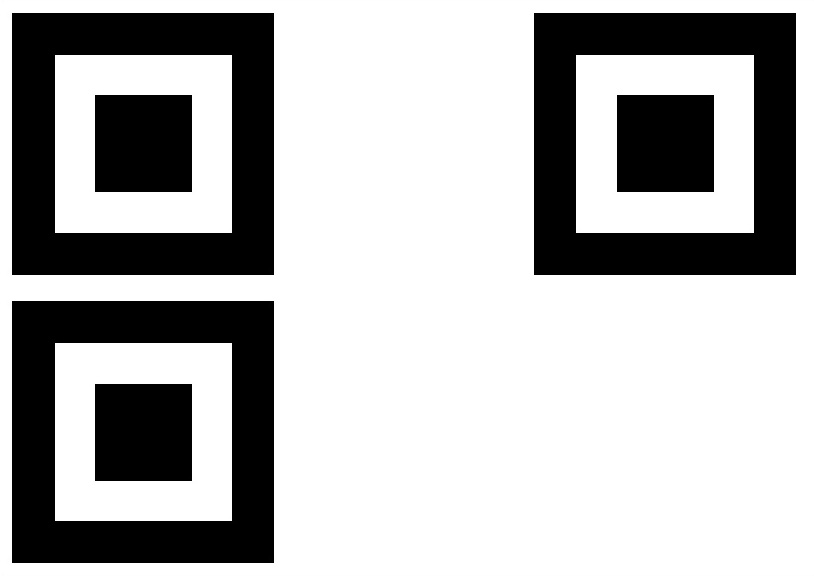
\includegraphics[width=0.35\textwidth]{./pics_camara/marcador.jpg}
	\end{center}
	\caption{Marcador utilizado}
	\label{fig:marcador}
\end{wrapfigure}

\section{Detección del marcador}

Para la detección del marcador se utilizará como base la detección de segmentos con el algoritmo \textbf{LSD} disponible en la página \url{http://www.ipol.im/pub/algo/gjmr_line_segment_detector/}.\\

Una vez detectados los segmentos se estudia cuáles de ellos pertenecen a estructuras formadas por 4 segmentos conexos y cerrados, es decir, se conservan solamente los segmentos pertenecientes a algún cuadrilátero. Posteriormente se realiza un nuevo filtrado dejando únicamente a las estructuras compuestas por 3 cuadrados concéntricos.\\

Una vez obtenidos los 3 bloques de 3 cuadrados concéntricos se utilizan todas las esquinas de todos los cuadrados para hallar la correspondencia entre las coordenadas del mundo y las esquinas detectadas en la foto. Se tienen así 36 puntos de correspondencias.\\

\begin{figure}[h!]
  \begin{center}
	\subfloat[Detección de segmentos: LSD]{\label{fig:lsd}
	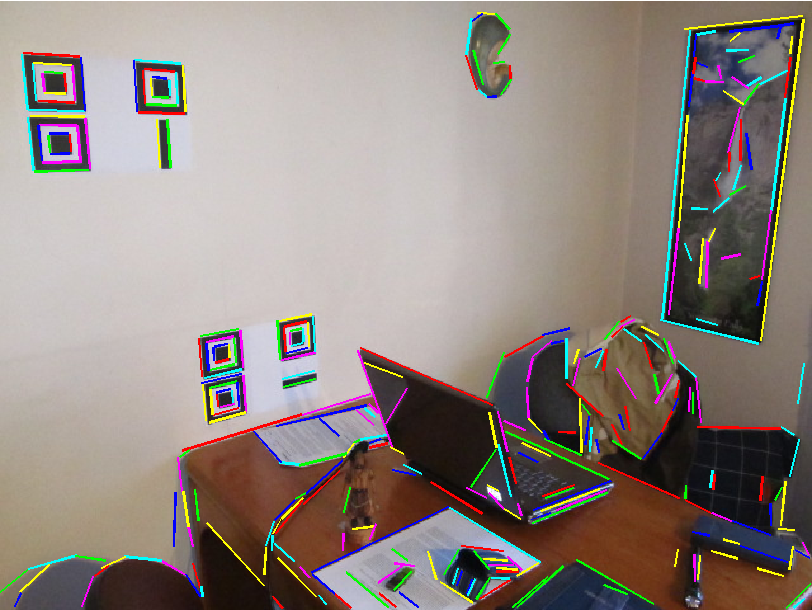
\includegraphics[width=0.5\textwidth]{./pics_camara/lsd.png}}
	\subfloat[Detección del marcador, filtrado del LSD]{\label{fig:lsd_filt}
	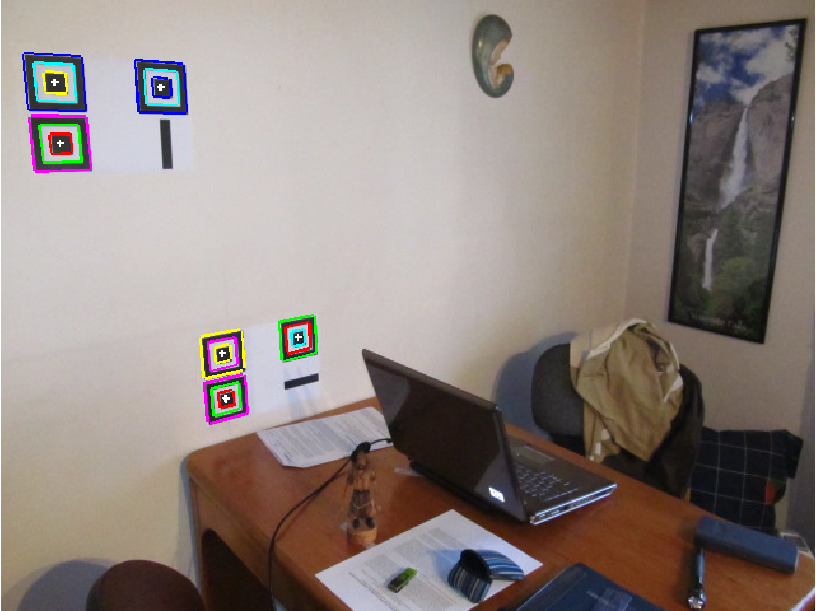
\includegraphics[width=0.5\textwidth]{./pics_camara/lsd_filt.png}}		
  \end{center}
  \caption{Detección y filtrado de segmentos}
  \label{fig:lsds}
\end{figure}

En la figura \ref{fig:lsds} se muestra una fotografía donde aparecen 2 marcadores distintos. Al aplicarle el detector de segmentos LSD se obtuvo la figura \ref{fig:lsd}. Luego se detectaron cuáles de estos segmentos pertenecen a estructuras como las descritas anteriormente (3 bloques de 3 cuadrados concéntricos corresponden a un marcador), y los resultados se muestran en la figura \ref{fig:lsd_filt}.\\

Por un lado es muy improbable obtener un falso positivo ya que los marcadores llevan una estructura muy particular, difícil de confundir. Por otro lado la debilidad de este método de detección está en poder detectar todos los segmentos de los 9 cuadrados involucrados. Es decir que si en la detección de segmentos no se detecta alguno de los 36 segmentos involucrados en los 9 cuadrados, el algoritmo no detectará ningún marcador.\\

Claramente se puede implementar algún tipo de algoritmo que introduzca cierta tolerancia, permitiendo que falten algunos segmentos. Esta sería una importante mejora a implementar ya que agrega una gran robustez al algoritmo.

\section{Resultados}

El lugar de la habitación donde se encuentra el marcador es conocido, entonces alcanza con obtener la posición relativa de la cámara respecto al marcador para obtener la posición de la cámara en relación a la habitación. Como ya se mencionó, existe una rotación \textbf{R} y una traslación \textbf{T} que llevan las coordenadas del mundo referenciadas en el marcador a las coordenadas del mundo referenciadas en la cámara. Entonces al obtener \textbf{R} y \textbf{T} estamos obteniendo la posición de la cámara. Observar que al transformar el origen de las coordenadas del mundo se obtienen unas coordenadas de la cámara iguales a T.\\

Como forma de verificar el buen funcionamiento del programa, se realizan pruebas en condiciones controladas, sabiendo con una precisión aceptable la verdadera posición relativa entre la cámara y el marcador. Se realizaron 7 pruebas en condiciones distintas, como se indica en la tabla \ref{tab:pruebas}.
\begin{table}[H]
\centering
\begin{tabular}{|c|c|c|c|c|} 
\hline \cellcolor[gray]{0.8} \textbf{Prueba} & \cellcolor[gray]{0.8} \textbf{Roll ($^o$)} & \cellcolor[gray]{0.8} \textbf{Pitch ($^o$)} & \cellcolor[gray]{0.8} \textbf{Yaw ($^o$)} & \cellcolor[gray]{0.8} \textbf{Z ($cm$)}\\ 
\hline 1 & 0   & 0   & 0   & 50 \\ 
\hline 2 & 0   & -30 & 0   & 50 \\ 
\hline 3 & -30 & 0   & 0   & 50 \\ 
\hline 4 & -30 & -30 & 0   & 50 \\ 
\hline 5 & 0   & 0   & -15 & 50 \\ 
\hline 6 & 0   & -30 & -15 & 50 \\ 
\hline 7 & 0   & 0   & 0   & 100 \\
\hline
\end{tabular} 
\caption{Pruebas realizadas}
\label{tab:pruebas}
\end{table}

Se muestran a continuación únicamente los resultados obtenidos para la prueba 5, ya que los resultados para el resto de las pruebas es muy similar.

\subsection{Prueba N$^o$ 5}

Al ejecutar el programa se obtiene la siguiente salida:

\begin{verbatim}
roll   = 357.34º
pitch  = 5.68º
yaw    = 342.97º
x      = -0.59mm
y      = -0.58mm
z      = 521.36mm
El marcador tiene en el 4o lugar una barra horizontal.
\end{verbatim}

Como se puede observar los resultados son muy aceptables, obteniendo un error de unos pocos grados en los ángulos, y apenas 2 centímetros en la posición. Además es importante destacar que se cometió un error sistemático en el proceso de adquisición ya que la distancia en el eje ``$z$'' se midió desde el marcador hasta el extremo del lente más cercano. En su lugar se debería haber considerado la distancia hasta donde se forma la imagen en la cámara, que es un tanto más adentro. Si se hubiera considerado este aspecto, la medida sería aún más fidedigna, ya que la distancia del lente al centro del plano de proyección sobre el que se forma la imagen en la cámara, sumaría un par de centímetros a la medida realizada.

\subsubsection*{Reproyección}

\begin{wrapfigure}{r}{0.5\textwidth}
	\begin{center}
	\vspace{-20pt}
		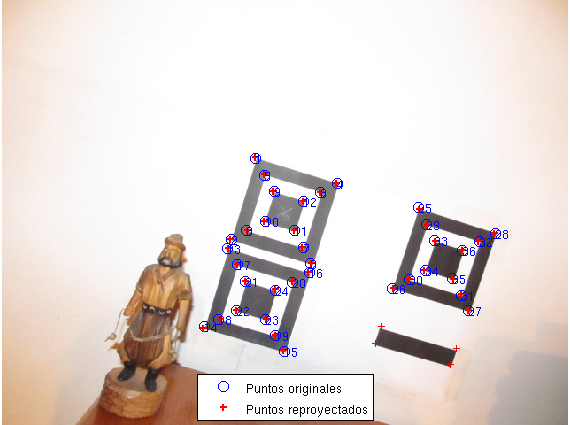
\includegraphics[width=0.45\textwidth]{./pics_camara/resultado_rp.png}
	\end{center}
	\caption{Reproyección de esquinas}
	\label{fig:resultado_rp}
\end{wrapfigure}

Este es quizás el método más confiable para determinar si los resultados obtenidos son correctos. En la figura \ref{fig:resultado_rp} se muestra con círculos azules las esquinas detectadas en la foto y con cruces rojas se indican la proyecciones de las coordenadas de la estructura 3D del marcador, utilizando las matrices \textbf{R} y \textbf{T} obtenidas. Puede verse claramente la cercanía entre los cículos azules y las cruces rojas, indicando que el conjunto de parámetros extrínsecos obtenidos son los correctos.\\

Es importante destacar, de todas maneras, que esta verificación no es 100\% confiable ya que pueden haber diferenctes combinaciones de parámetros intrínsecos de la cámara que determinen la misma reproyección. Por ejemplo los siguientes 2 juegos de parámetros:
\begin{itemize}
\item Field of view = A   ; Distancia = B
\item Field of view = A/2 ; Distancia = 2*B
\end{itemize}

\subsubsection*{Ploteo de la posición relativa}

Consiste en una herramienta gráfica que permite verificar a grandes rasgos si los resultados son coherentes con la realidad.\\
 
\begin{figure}
  \begin{center}
	\subfloat[Cámara fija]{\label{fig:resultado_cf}
	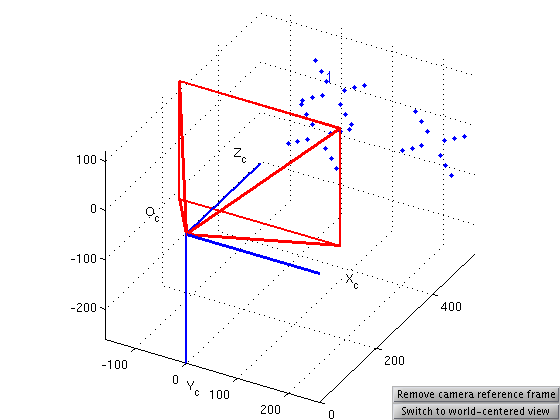
\includegraphics[width=0.5\textwidth]
		{./pics_camara/resultado_cf.png}}
	\subfloat[Marcador fijo]{\label{fig:resultado_mf}
	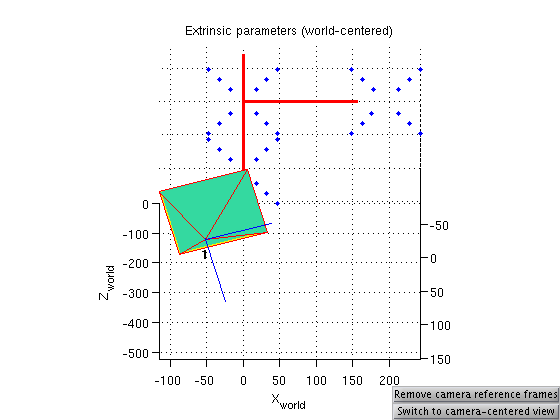
\includegraphics[width=0.5\textwidth]
		{./pics_camara/resultado_mf.png}}		
  \end{center}
  \caption{Ploteo de posición y orientación obtenida}
  \label{fig:plots}  
\end{figure}

En la figura \ref{fig:plots} se presentan 2 imágenes: la primera basada en las coordenadas de la cámara, es decir dejando la cámara fija y ubicando el marcador y la segunda basada en las coordenadas del mundo, es decir dejando el marcador fijo y ubicando la posición relativa de la cámara.

\subsubsection*{Realidad aumentada}

\begin{wrapfigure}{l}{0.55\textwidth}
	\begin{center}
		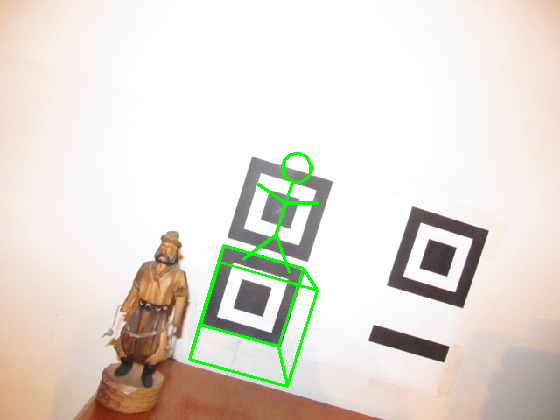
\includegraphics[width=0.5\textwidth]{./pics_camara/resultado_ar.png}
	\end{center}
	\caption{Realidad aumentada}
	\label{fig:resultado_ar}
\end{wrapfigure}

Por último y a modo didáctico, se presenta un ejemplo de Realidad Aumentada. Se trata de proyectar en la imagen una estructura tridimensional como si estuviera en la habitación. Resulta interesante ya que se puede apreciar con claridad la perspectiva con la que está mirando al marcador y analizar si la perspectiva del objeto añadido se corresponde.\\

Se añade un cubo con una de las caras coincidente con uno de los cuadrados del marcador, y sobre el aparece parado un fosforito. Los resultados se pueden apreciar en la figura \ref{fig:resultado_ar}.\\[25pt]

\underline{Nota general:} Si bien el algoritmo fue implementado y testeado, todo el trabajo fue realizado en $MatLab$. Por razones del tiempo acotado del proyecto no se puedo portar el código a $C$, quedando como trabajo a ser realizado en el futuro. A su vez se cuenta con todo el hardware necesario para su implementación ya que la $BeagleBoard$ tiene capacidad para procesar video en tiempo real, cuenta con librerías especiales para el tratamiento de imágenes y se adquirió una cámara pensada para la placa que tiene las ventajas de un fácil montaje y compatibilidad asegurada.

%\end{document}